


\documentclass[journal,12pt,onecolumn,draftclsnofoot]{IEEEtran}


\usepackage{amsthm}
\usepackage{amsmath}
\usepackage{amssymb}
\usepackage{booktabs}
\usepackage{color}
\usepackage{epsfig}
\usepackage{subfigure}
\usepackage{graphicx}
%\usepackage{caption}
\usepackage{colortbl}

\renewcommand{\arraystretch}{1.3} 
\newcommand{\diag}{\mathop{\mathrm{diag}}}
\newcommand{\tabincell}[2]{\begin{tabular}{@{}#1@{}}#2\end{tabular}}  

\newtheorem{assumption}{\textbf{Assumption}}
\newtheorem{definition}{\textbf{Definition}}
\newtheorem{lemma}{\textbf{Lemma}}
\newtheorem{theorem}{\textbf{Theorem}}
\newtheorem{remark}{\textbf{Remark}}
\newtheorem{proposition}{\textbf{Proposition}}
\newtheorem{corollary}{\textbf{Corollary}}

\def\ba{\begin{array}}
	\def\ea{\end{array}}
\newcommand{\beq}{\begin{equation}}
\newcommand{\eeq}{\end{equation}}
\newcommand{\bq}{\begin{eqnarray}}
\newcommand{\eq}{\end{eqnarray}}
\newcommand{\bqn}{\begin{eqnarray*}}
	\newcommand{\eqn}{\end{eqnarray*}}
\newcommand{\bee}{\begin{enumerate}}
	\newcommand{\eee}{\end{enumerate}}
\newcommand{\bi}{\begin{itemize}}
	\newcommand{\ei}{\end{itemize}}
%\newcommand{\qed}{\hfill{$\blacksquare$}}
\newcommand{\ii}{\textbf{i}}

\usepackage{comment}
%\newboolean{showcomments}
%\setboolean{showcomments}{true}
\newcommand{\slow}[1]{\ifthenelse{\boolean{showcomments}}
	{ \textcolor{red}{(SL:  #1)}}{}}
\newcommand{\you}[1]{\ifthenelse{\boolean{showcomments}}
	{ \textcolor{green}{(PCY:  #1)}}{}}
\newcommand{\john}[1]{\ifthenelse{\boolean{showcomments}}
	{ \textcolor{blue}{(jp:  #1)}}{}}


% correct bad hyphenation here
\hyphenation{op-tical net-works semi-conduc-tor}


\begin{document}

%\title{Question}


%\author{Pengcheng You \\  Nov 14 2017% <-this % stops a space
%\thanks{M. Shell was with the Department
%of Electrical and Computer Engineering, Georgia Institute of Technology, Atlanta,
%GA, 30332 USA e-mail: (see http://www.michaelshell.org/contact.html).}% <-this % stops a space
%\thanks{J. Doe and J. Doe are with Anonymous University.}% <-this % stops a space
%\thanks{Manuscript received April 19, 2005; revised August 26, 2015.}
%}


% make the title area
%\maketitle


%\begin{abstract}
%
%\end{abstract}

%
%\begin{IEEEkeywords}
%
%\end{IEEEkeywords}


\IEEEpeerreviewmaketitle

\noindent
\textbf{Bang control}

Fig.~\ref{fig:bangcontrol} shows the bang control, or load shedding strategy, when the frequency drops below a threshold. Here I set the threshold to 59.9 Hz for illustrative purpose. Initially there is a negative step change of power deficiency in the network. Therefore the frequency starts to drop. When the threshold is reached, a unit (100MW) of load shedding is modeled by a positive step change of power injection at the bus with the lowest frequency. In Fig.~\ref{fig:bang_freq} additional fluctuations can observed at the point of bang control (orange in contrast to purple). After bang control, the frequency trajectories tend to be more mild compared with those without bang control in Fig.~\ref{fig:bang_normal_freq}. Overall the difference is not obvious. The linear controller seems very robust to the step changes of power imbalance. The intuition may be in the linear model the controller is proven globally asymptotically stable.

Another interesting observation is that the impact of load shedding on frequency doesn't take effect instantly. As Fig.~\ref{fig:bang_freq} shows, the bang control doesn't raise frequency immediately, maybe due to the large inertia of the whole system, but it indeed make the trajectories less fluctuating.

\begin{figure}
	\centering
\subfigure[]{
		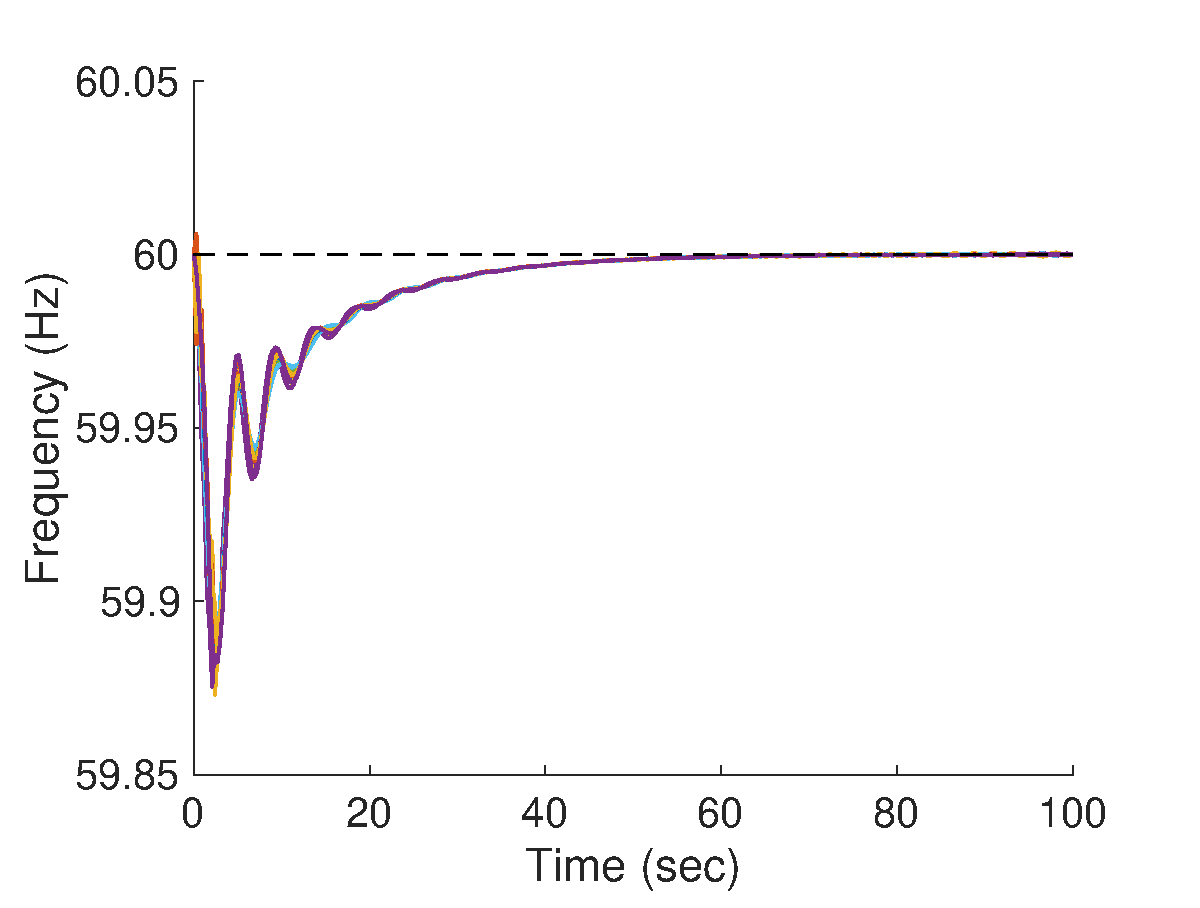
\includegraphics[width=0.45\linewidth]{figures/bang_freq.eps}
		\label{fig:bang_freq}
	}
\subfigure[]{
	\includegraphics[width=0.45\linewidth]{figures/normal_freq.eps}
	\label{fig:bang_normal_freq}
}
\caption{(a) Bang control: load shedding (positive step change of imbalance) when frequency drops below 59.9 Hz; (b) Without bang control.}
\label{fig:bangcontrol}
\end{figure}

\noindent
\textbf{Spoofing}

In terms of spoofing, Enoch first suggested a simple strategy $P=P_0+\frac{\alpha}{P_{\text{real}}}$. My major concern about this strategy is that $P$ is negatively correlated with $P_{\text{real}}$. This may make the spoofing easily detectable as the system states will evolve in a direction opposite to what is expected. Instead, I tried a simple variant $P=P_0-\frac{\alpha}{P_{\text{real}}}$ to make the state evolution in the consistent direction. The results are shown in Fig.~\ref{fig:spoofed1}. Two drawbacks about this spoofing strategy: (a) the spoof price $P$ will explode when $P_{\text{real}}$ approaches 0; (b) when $|P_{\text{real}}|$ is large, $P_0$ is the dominant term. It remains a problem how to set $P_0$. In my simulations, I played a trick to set $P_0$ to the original equilibrium price with the benefit of hindsight such that the final price only deviates a little bit. Therefore, as Fig.~\ref{fig:spoofed1_freq} shows, the frequency is still around the nominal value with a small shift. In addition, since $P_0$ dominates the second term in $P$, $P$ approximates $P_0$ from the beginning (see Fig.~\ref{fig:spoofed1_dlmp}), thus accelerating the convergence. However, it is not implementable in practice to set $P_0$ in this way.

\begin{figure}
	\centering
	\subfigure[]{
		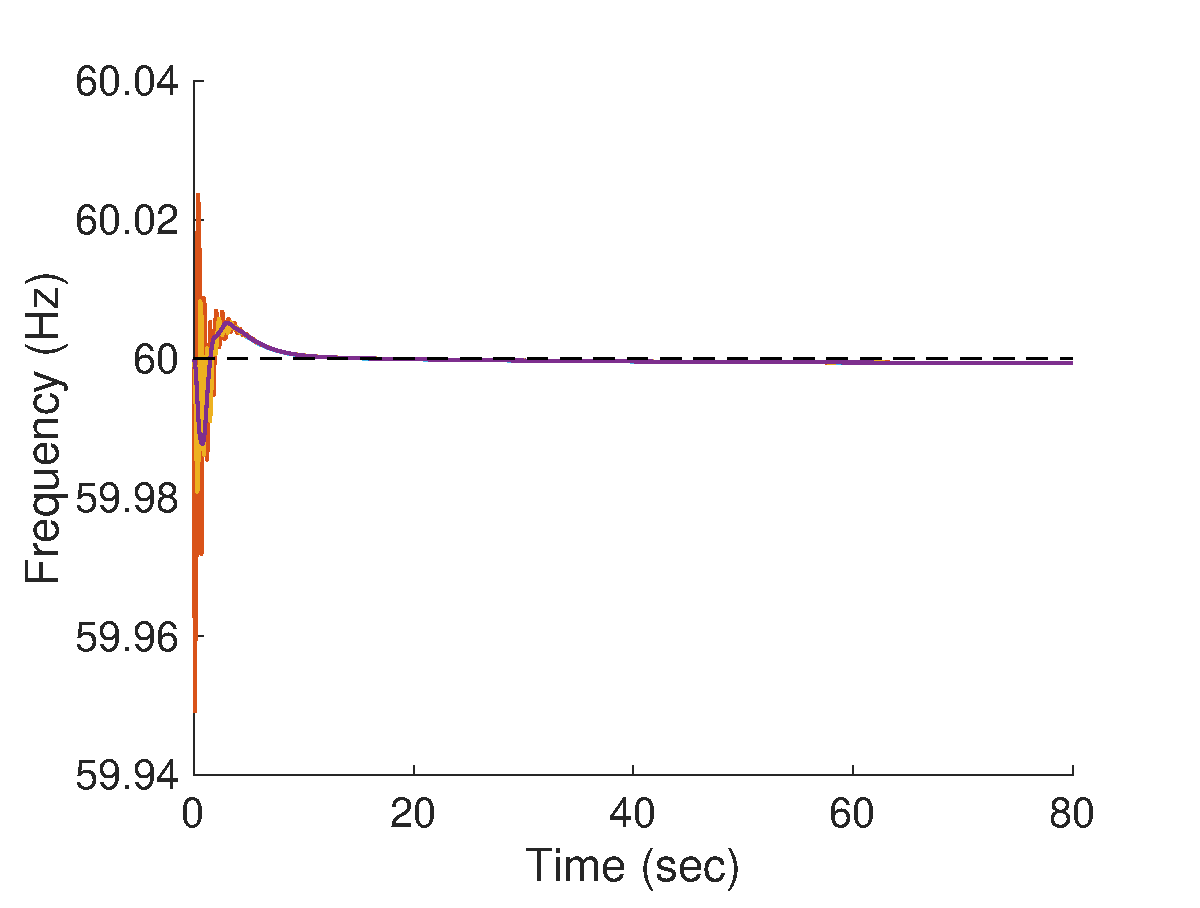
\includegraphics[width=0.45\linewidth]{figures/result_spoofingdesign1/spoofed_freq.eps}
		\label{fig:spoofed1_freq}
	}
	\subfigure[]{
		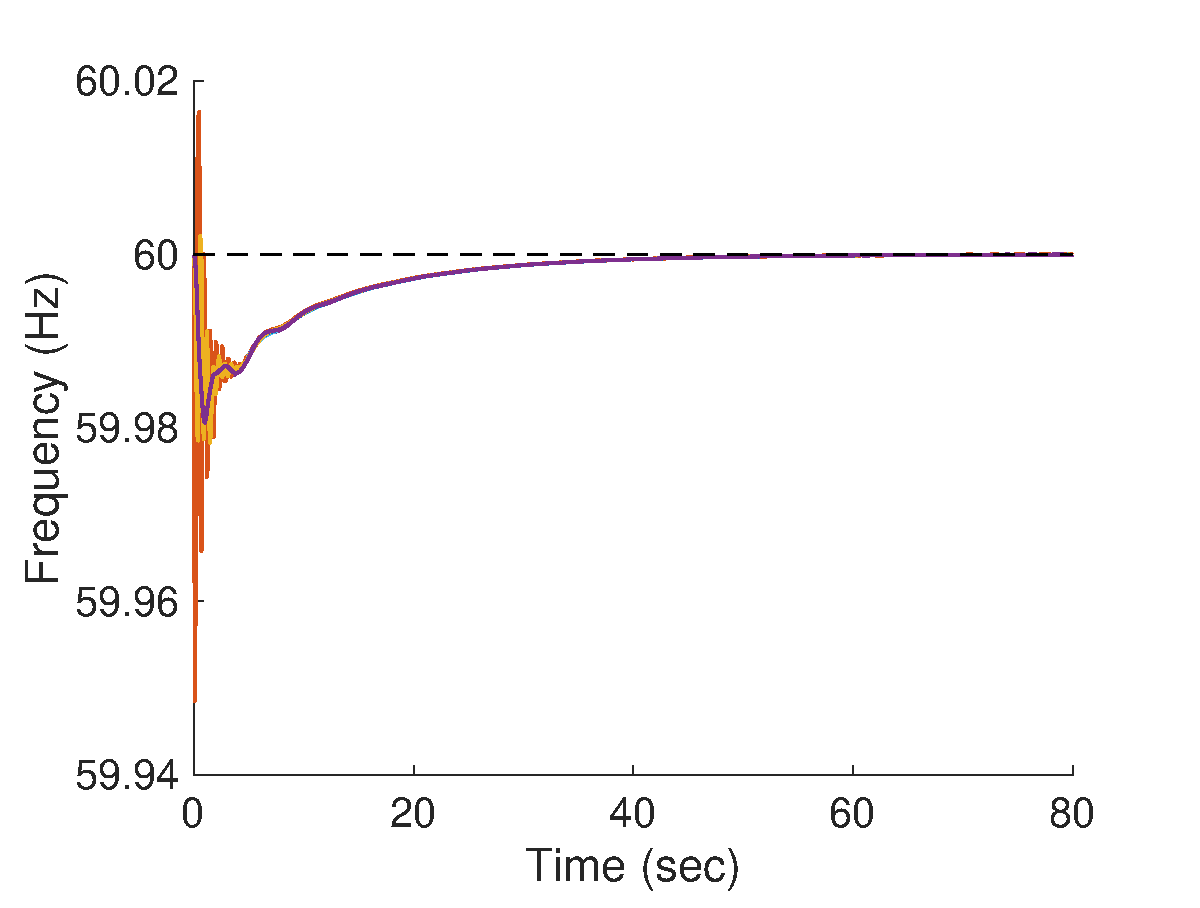
\includegraphics[width=0.45\linewidth]{figures/result_spoofingdesign1/normal_freq.eps}
		\label{fig:spoofed1_normal_freq}
	}
	\subfigure[]{
	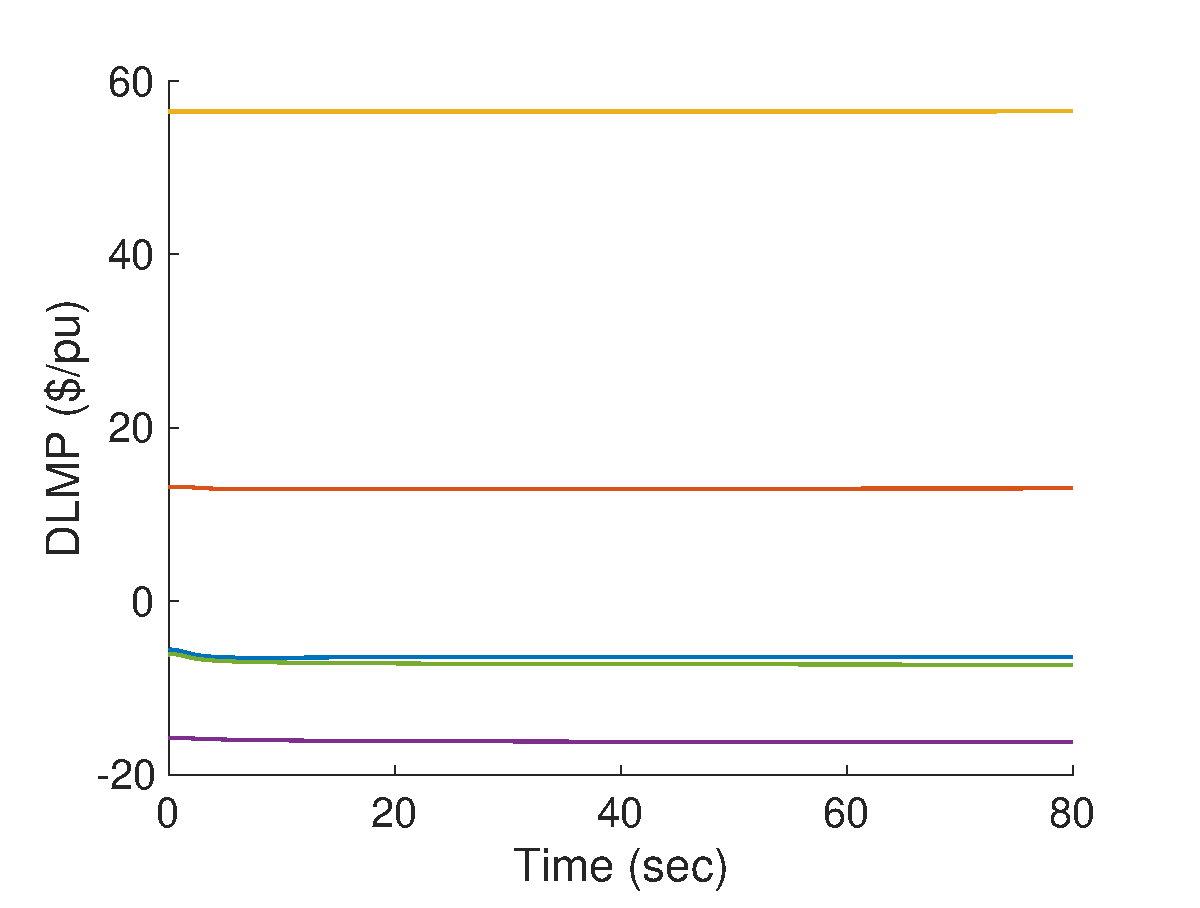
\includegraphics[width=0.45\linewidth]{figures/result_spoofingdesign1/spoofed_DLMP.eps}
	\label{fig:spoofed1_dlmp}
}
\subfigure[]{
	\includegraphics[width=0.45\linewidth]{figures/result_spoofingdesign1/normal_DLMP.eps}
	\label{fig:spoofed1_normal_dlmp}
}
	\caption{Spoofing strategy $P=P_0-\frac{\alpha}{P_{\text{real}}}$: (a) frequency; (b) normal frequency; (c) DLMP; (d) normal DLMP. }
	\label{fig:spoofed1}
\end{figure}

To avoid the above problems, I came up with a new spoofing strategy $P=P_{\text{real}}+\frac{\alpha}{\overline{P} - P_{\text{real}}}$. The parameter $\overline{P}$ is an upper bound of prices, which can be set based on all past prices such that $P_{\text{real}}$ won't approach $\overline{P}$ with a certain gap. Therefore, the spoof price $P$ always upper bound $P_{\text{real}}$ and the smaller $P_{\text{real}}$ is, the more accurately $P$ approximates $P_{\text{real}}$ (We can also set the opposite way using a price lower bound $\underline{P}$ ). Besides, $P$ evolves in the same direction as $P_{\text{real}}$. The test result is shown in Fig.~\ref{fig:spoofed2}, where I set $\alpha=500$ and $\overline{P}=[50\ 15\ 15\ 15\ 15]$. Surprisingly, with the spoofing strategy the frequency still converges to its nominal value, which can be loosely explained by the fact that $\dot P = 0 \leftrightarrow \dot P_{\text{real}} = 0 $. However, actually the DLMPs at equilibrium are different from those without spoofing, as Fig.~\ref{fig:spoofed2_dlmp} and Fig.~\ref{fig:spoofed2_normal_dlmp} suggest. If this is correct, this spoofing strategy is a good one in the sense that it doesn't disrupt or even deviate the frequency, which makes it less detectable, but enforces the system operating point to deviate from the optimal one, thus suffering a economic loss.

\begin{figure}
	\centering
	\subfigure[]{
		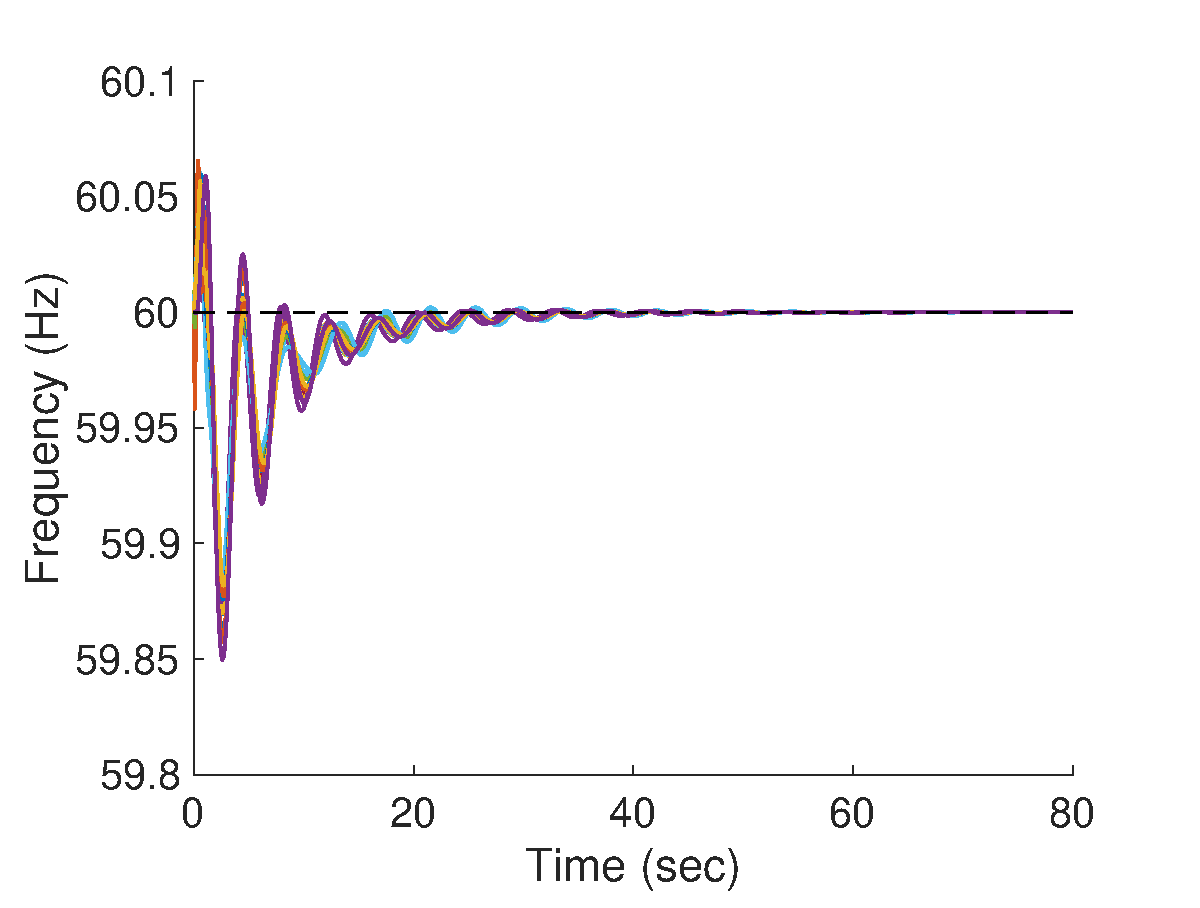
\includegraphics[width=0.45\linewidth]{figures/result_spoofingdesign2/spoofed_freq.eps}
		\label{fig:spoofed2_freq}
	}
	\subfigure[]{
		\includegraphics[width=0.45\linewidth]{figures/result_spoofingdesign2/normal_freq.eps}
		\label{fig:spoofed2_normal_freq}
	}
	\subfigure[]{
		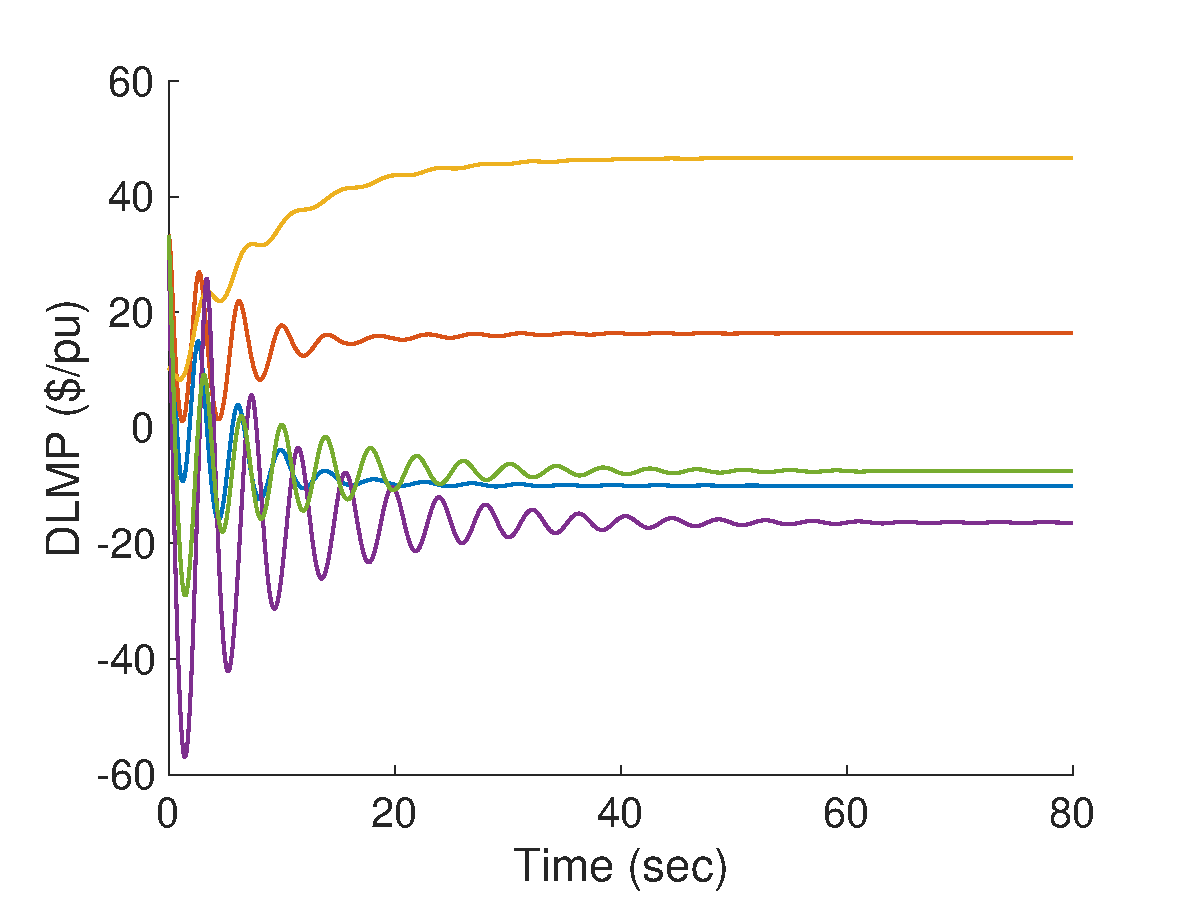
\includegraphics[width=0.45\linewidth]{figures/result_spoofingdesign2/spoofed_DLMP.eps}
		\label{fig:spoofed2_dlmp}
	}
	\subfigure[]{
		\includegraphics[width=0.45\linewidth]{figures/result_spoofingdesign2/normal_DLMP.eps}
		\label{fig:spoofed2_normal_dlmp}
	}
	\caption{Spoofing strategy $P=P_{\text{real}}+\frac{\alpha}{\overline{P} - P_{\text{real}}}$: (a) frequency; (b) normal frequency; (c) DLMP; (d) normal DLMP. }
	\label{fig:spoofed2}
\end{figure}







%\bibliographystyle{IEEEtran}  
%\bibliography{bib}  


\end{document}


